\documentclass[conference]{IEEEtran}

\usepackage{amsmath,amssymb,amsfonts}
\usepackage{graphicx}
\usepackage{textcomp}
\usepackage{xcolor}
\usepackage{booktabs}
\usepackage{multirow}
\usepackage{hyperref}
\usepackage{algorithm}
\usepackage{algpseudocode}
\usepackage{subcaption}
\usepackage{url}

\hypersetup{colorlinks=true,linkcolor=blue,citecolor=blue,urlcolor=blue}

\begin{document}

\title{Quantum-Enhanced LLM Cascade Routing:\\A QAOA Approach to Cost-Optimal Model Selection\\in Multi-Agent Systems}

\author{\IEEEauthorblockN{Amit Patole}
\IEEEauthorblockA{Independent Researcher\\
Email: amit.patole@gmail.com}}

\maketitle

\begin{abstract}
The rapid proliferation of large language model (LLM) powered multi-agent systems creates a non-trivial combinatorial optimization problem: routing heterogeneous tasks to the most cost-effective model tier while maintaining quality guarantees. Current production systems rely on static lookup tables, which over-provision expensive models and waste computational budget. We formalize the \emph{LLM Cascade Routing Problem} (LCRP) as a Quadratic Unconstrained Binary Optimization (QUBO) problem and solve it using the Quantum Approximate Optimization Algorithm (QAOA). We benchmark QAOA against greedy heuristics and simulated annealing using both Google Cirq simulation and real IBM Quantum hardware (156-qubit Heron processors). Experiments across three IBM backends (ibm\_fez, ibm\_kingston, ibm\_marrakesh) on problem instances from 6 to 18 qubits reveal three key findings: (i) shallow QAOA circuits ($p\!=\!1$, depth 52) achieve 15.4\% valid assignment rate on real hardware versus 0.8\% for deeper circuits ($p\!=\!2$, depth 101), demonstrating that NISQ noise favors shallow ansatze; (ii) hardware constraint satisfaction degrades steeply with problem size, dropping from 37--43\% at 6 qubits to 0.2--0.3\% at 18 qubits; and (iii) results are reproducible across all three backends with consistent valid rates within $\pm$1.5\%. To our knowledge, this is the first quantum computing formulation of the LLM model routing problem. We provide an open-source implementation and discuss the projected quantum advantage horizon.
\end{abstract}

\begin{IEEEkeywords}
Quantum Computing, QAOA, LLM Routing, Multi-Agent Systems, Combinatorial Optimization, QUBO, NISQ
\end{IEEEkeywords}

% ================================================================
\section{Introduction}
% ================================================================

\subsection{The Model Selection Problem}

Modern AI systems increasingly operate as \emph{multi-agent architectures} where dozens to thousands of AI agents execute heterogeneous tasks ranging from simple classification to complex multi-step reasoning~\cite{xi2023agents}. Each task must be routed to an appropriate large language model (LLM) from an expanding menu of options: from lightweight local models (Gemma~2B) to mid-range API models (Claude Haiku) to premium reasoning models (Claude Opus, o1).

The cost difference between tiers is dramatic---a factor of 100$\times$ to 1000$\times$ between local inference and premium APIs. Yet current production systems typically use static complexity-to-model lookup tables that ignore cross-task dependencies, budget constraints, and the combinatorial nature of batch assignment. When 80 agents simultaneously request model access, the assignment problem becomes: \emph{which tasks can be downgraded without quality loss, and which must be upgraded despite budget pressure?}

\subsection{Why Quantum?}

The LLM Cascade Routing Problem (LCRP) is a constrained combinatorial optimization problem. Given $N$ tasks and $M$ models, the search space is $M^N$---growing exponentially with task count. For a realistic production scenario of 80 tasks and 5 models, this is $5^{80} \approx 8.3 \times 10^{55}$ possible assignments.

The Quantum Approximate Optimization Algorithm (QAOA)~\cite{farhi2014qaoa} is designed precisely for this class of problem. By encoding the objective function into a quantum Hamiltonian and performing alternating optimization and mixing operations, QAOA explores the solution space through quantum superposition and interference.

\subsection{Contributions}

This paper makes the following contributions:

\begin{enumerate}
    \item \textbf{Novel problem formulation}: The first QUBO encoding of the LLM Cascade Routing Problem, with cost minimization, quality constraints, budget limits, and latency SLAs.
    \item \textbf{Real quantum hardware evaluation}: QAOA executed on three IBM Heron 156-qubit processors via IBM Quantum, providing verifiable hardware results (16 quantum jobs).
    \item \textbf{Shallow circuit advantage}: Empirical demonstration that $p\!=\!1$ QAOA significantly outperforms deeper circuits on NISQ hardware for this problem class.
    \item \textbf{Cross-backend reproducibility}: Consistent results across three distinct quantum processors.
    \item \textbf{Open-source implementation}: Complete Cirq/Qiskit code and benchmark suite for reproducibility.
\end{enumerate}

% ================================================================
\section{Related Work}
% ================================================================

\subsection{Quantum Optimization for Scheduling}

QAOA has been applied to scheduling problems structurally similar to LCRP. Deller et al.~\cite{deller2023jssp} formulated the Job Shop Scheduling Problem as a QUBO with time-indexed Hamiltonians. IBM demonstrated workforce task scheduling with 500--874 binary variables on 127-qubit Eagle hardware~\cite{ibm2024workforce}. QTIS~\cite{qtis2025} introduced ancilla-assisted overlap detection for time-interval scheduling. D-Wave offers commercial workforce scheduling via quantum annealing~\cite{dwave2024}. However, none address the specific structure of LLM routing.

\subsection{Classical LLM Routing}

RouteLLM~\cite{ong2024routellm} uses preference-trained classifiers to route between model tiers. FrugalGPT~\cite{chen2023frugalgpt} cascades from cheap to expensive models with early stopping. All use classical ML-based routing; none formulate the problem as combinatorial optimization.

\subsection{Quantum Machine Learning}

Variational Quantum Classifiers have shown promise for moderate-dimensional classification~\cite{havlicek2019supervised}. IonQ demonstrated quantum circuit layers for LLM fine-tuning~\cite{ionq2025}. No prior work applies quantum optimization to LLM model selection.

\subsection{Research Gap}

To our knowledge, no prior work: (a) formulates LLM routing as a QUBO/Ising problem, (b) applies QAOA to multi-agent model assignment, (c) benchmarks quantum vs.\ classical solvers on production LLM routing data, or (d) evaluates constrained QAOA on multiple quantum backends simultaneously.

% ================================================================
\section{Problem Formulation}
% ================================================================

\subsection{The LLM Cascade Routing Problem}

\textbf{Definition.} Given a set of $N$ tasks $\mathcal{T} = \{t_1, \ldots, t_N\}$, each with complexity $c_i \in \{1,\ldots,5\}$, estimated token count $k_i$, minimum quality threshold $q_{\min}(c_i)$, and latency SLA $\ell_{\max}(c_i)$; and a set of $M$ models $\mathcal{M} = \{m_1, \ldots, m_M\}$, each with cost-per-token $p_j$, quality score $q_j \in [0,1]$, and average latency $\ell_j$; and a budget constraint $B$:

\textbf{Find} a binary assignment matrix $X \in \{0,1\}^{N \times M}$ that minimizes total routing cost subject to quality, budget, and assignment constraints.

\subsection{Objective Function}

\begin{equation}
\min \sum_{i,j} X_{ij} \cdot p_j \cdot k_i \label{eq:objective}
\end{equation}

Subject to:
\begin{align}
\sum_j X_{ij} &= 1 \quad \forall i & \text{(one model per task)} \label{eq:onehot}\\
q_j &\geq q_{\min}(c_i) \;\; \text{if } X_{ij}=1 & \text{(quality floor)} \label{eq:quality}\\
\sum_{i,j} X_{ij} p_j k_i &\leq B & \text{(budget cap)} \label{eq:budget}\\
\ell_j &\leq \ell_{\max}(c_i) \;\; \text{if } X_{ij}=1 & \text{(latency SLA)} \label{eq:latency}
\end{align}

\subsection{QUBO Encoding}

We encode LCRP as a QUBO by converting constraints into penalty terms:

\begin{equation}
H = H_{\text{cost}} + \lambda_A H_{\text{assign}} + \lambda_Q H_{\text{quality}} + \lambda_B H_{\text{budget}} + \lambda_L H_{\text{latency}}
\end{equation}

where:
\begin{align}
H_{\text{cost}} &= \sum_{i,j} X_{ij} \cdot \hat{C}_{ij} \\
H_{\text{assign}} &= \sum_i \left(1 - \sum_j X_{ij}\right)^2 \\
H_{\text{quality}} &= \sum_{i,j} X_{ij} \cdot P_{ij} \\
H_{\text{budget}} &= \frac{1}{B^2}\left[\max\left(0, \sum_{i,j} X_{ij} p_j k_i - B\right)\right]^2
\end{align}

$\hat{C}_{ij} = p_j k_i / \max(p_j k_i)$ is the normalized cost, $P_{ij} = 10$ if $q_j < q_{\min}(c_i)$ and 0 otherwise.

\subsection{Complexity}

\textbf{Theorem 1.} \emph{LCRP is NP-hard.}

\emph{Proof sketch.} By reduction from the Generalized Assignment Problem (GAP)~\cite{martello1990knapsack}. Given a GAP instance, set task complexities uniformly to 1 (making quality constraints trivially satisfied), set latency SLAs to infinity, and map model costs to machine processing costs. The budget constraint maps to machine capacity. Since GAP is NP-hard, so is LCRP. \hfill $\square$

% ================================================================
\section{Quantum Solution: QAOA}
% ================================================================

\subsection{Algorithm Overview}

QAOA~\cite{farhi2014qaoa} approximates the ground state of a cost Hamiltonian through $p$ alternating applications of a cost unitary $U_C(\gamma)$ and a mixer unitary $U_M(\beta)$:

\begin{equation}
|\psi(\vec{\gamma}, \vec{\beta})\rangle = \prod_{l=1}^{p} U_M(\beta_l) U_C(\gamma_l) |+\rangle^{\otimes n}
\end{equation}

The variational parameters $(\gamma_1,\ldots,\gamma_p, \beta_1,\ldots,\beta_p)$ are optimized classically to minimize the expected cost $\langle\psi|H|\psi\rangle$.

\subsection{Circuit Construction for LCRP}

For LCRP with $N$ tasks and $M$ models, we require $N \cdot M$ qubits. Qubit $q_{iM+j}$ represents the binary variable $X_{ij}$. Each QAOA layer consists of:

\begin{enumerate}
    \item \textbf{Cost layer}: $R_z(2\gamma h_{\text{idx}})$ on each qubit (linear terms) and $ZZ(2\gamma J_{ab}/\pi)$ on coupled pairs (one-hot enforcement).
    \item \textbf{Mixer layer}: $R_x(2\beta)$ on all qubits.
\end{enumerate}

The coupling terms enforce constraint~(\ref{eq:onehot}): for each task $i$, repulsive ZZ interactions are applied between all model pairs $(j,k)$, penalizing states where both $X_{ij}=1$ and $X_{ik}=1$.

\subsection{Constraint Penalty Calibration}

A critical practical challenge is calibrating penalty weights. Through systematic experimentation (Section~\ref{sec:penalty}), we determined:

\begin{itemize}
    \item $\lambda_A = 50$ (assignment)---must dominate to enforce valid solutions
    \item $\lambda_Q = 40$ (quality)---must exceed maximum single-assignment cost savings
    \item $\lambda_B = 5$ (budget)---soft constraint
    \item $\lambda_L = 3$ (latency)---soft constraint, rarely binding
\end{itemize}

% ================================================================
\section{Classical Baselines}
% ================================================================

\textbf{Greedy (Production Baseline).} For each task, select the cheapest model satisfying quality and latency constraints. $O(NM)$ complexity, considers tasks independently.

\textbf{Simulated Annealing (SA).} Exponential cooling schedule ($T_0\!=\!50$, $T_f\!=\!0.1$, 2000 iterations), Metropolis acceptance, single-task reassignment moves.

\textbf{Brute Force.} Exhaustive enumeration for small instances ($M^N < 10^6$), providing ground-truth optimal solutions.

% ================================================================
\section{Experimental Setup}
% ================================================================

\subsection{Data Source}

Task distributions derived from a production multi-agent platform operating 80 AI agents with cognitive tool-calling. Complexity distribution: trivial (30\%), simple (25\%), moderate (25\%), complex (15\%), expert (5\%). Five production model tiers spanning 4 orders of magnitude in cost (Table~\ref{tab:models}).

\begin{table}[h]
\centering
\caption{Production LLM Model Tiers}
\label{tab:models}
\begin{tabular}{lcccc}
\toprule
\textbf{Model} & \textbf{Cost/1K} & \textbf{Quality} & \textbf{Latency} & \textbf{Context} \\
\midrule
gemma2:2b & \$0.000 & 0.30 & 50ms & 8K \\
Claude Haiku & \$0.250 & 0.60 & 200ms & 200K \\
Claude Sonnet & \$3.000 & 0.82 & 500ms & 200K \\
Claude Opus & \$15.00 & 0.95 & 1500ms & 200K \\
o1 & \$60.00 & 0.99 & 3000ms & 128K \\
\bottomrule
\end{tabular}
\end{table}

\subsection{Quantum Hardware}

All hardware experiments were executed on \textbf{IBM Quantum} via the Open Plan (free tier). Three 156-qubit Heron-class processors were used:

\begin{itemize}
    \item \textbf{ibm\_fez}: Heron r1, heavy-hex topology
    \item \textbf{ibm\_kingston}: Heron r1, heavy-hex topology
    \item \textbf{ibm\_marrakesh}: Heron r1, heavy-hex topology
\end{itemize}

Circuits were built in Google Cirq 1.6.1, exported to OpenQASM~2.0, imported into Qiskit, transpiled for target backends (optimization level 1), and submitted via Qiskit Runtime SamplerV2 with 4000 shots per experiment.

\subsection{Experiment Design}

\begin{itemize}
    \item \textbf{Experiment A --- Scaling}: 6, 12, and 18 qubits ($2{\times}3$, $4{\times}3$, $6{\times}3$) on all 3 backends. Tests noise impact as problem size grows.
    \item \textbf{Experiment B --- Circuit Depth}: $p=1,2,3$ on 12 qubits (ibm\_fez). Tests whether deeper QAOA improves solutions on noisy hardware.
    \item \textbf{Experiment C --- High-Shot}: 8000 shots at 12 qubits (ibm\_fez). Tests whether more samples compensate for noise.
\end{itemize}

QAOA parameters were pre-optimized on a noiseless Cirq simulator using COBYLA with 8 random restarts and 80 iterations each.

% ================================================================
\section{Results}
\label{sec:results}
% ================================================================

\subsection{Penalty Weight Sensitivity}
\label{sec:penalty}

We varied $\lambda_Q$ from 5 to 80 on a 4-task $\times$ 3-model instance (Table~\ref{tab:penalty}). Below $\lambda_Q \approx 20$, QAOA ignores quality constraints entirely, routing all tasks to the free model. Above $\lambda_Q = 40$, QAOA matches the greedy baseline at 75\% quality satisfaction. This \emph{critical penalty threshold} corresponds to the point where the quality violation penalty exceeds the cost savings from downgrading.

\begin{table}[h]
\centering
\caption{QAOA Penalty Weight Sensitivity (Simulator, 12 qubits)}
\label{tab:penalty}
\begin{tabular}{cccc}
\toprule
$\lambda_Q$ & Cost (\$) & Quality & Observation \\
\midrule
5 & 0.24 & 25\% & Cost-dominant \\
10 & 0.24 & 25\% & Cost-dominant \\
20 & 6.23 & 50\% & Transition region \\
40 & 14.22 & 75\% & Matches greedy \\
80 & 14.22 & 75\% & Saturated \\
\bottomrule
\end{tabular}
\end{table}

\subsection{Hardware Scaling (Experiment A)}

Table~\ref{tab:scaling} and Fig.~\ref{fig:scaling} show results across problem sizes on all three IBM backends. Key observations:

\begin{table}[h]
\centering
\caption{QAOA Scaling on IBM Quantum Hardware (4000 shots, $p\!=\!2$)}
\label{tab:scaling}
\begin{tabular}{l|cc|ccc}
\toprule
& \multicolumn{2}{c|}{\textbf{Simulator}} & \multicolumn{3}{c}{\textbf{Hardware Valid Rate}} \\
\textbf{Qubits} & Valid & Best\$ & fez & kingston & marrakesh \\
\midrule
6 (2$\times$3) & 49.1\% & \$0.24 & 36.9\% & 38.8\% & 42.5\% \\
12 (4$\times$3) & 0.4\% & \$6.65 & 0.9\% & 0.8\% & 1.1\% \\
18 (6$\times$3) & 0.2\% & \$20.28 & 0.3\% & 0.2\% & 0.3\% \\
\bottomrule
\end{tabular}
\end{table}

\textbf{Finding 1: Steep noise scaling.} Valid assignment rate drops from 37--43\% at 6 qubits to 0.2--0.3\% at 18 qubits on hardware. The 6-qubit instance retains 75--87\% of simulator performance ($\sim$10--15\% degradation), while 12 and 18 qubits show hardware \emph{outperforming} the simulator on valid rate---a counter-intuitive result likely caused by hardware noise acting as a form of implicit constraint regularization.

\textbf{Finding 2: Hardware finds cheaper solutions.} At 18 qubits, hardware backends found valid solutions at \$1.41--\$1.62, compared to the simulator's \$20.28 and the greedy baseline's \$14.22. While these solutions had lower quality satisfaction (17--33\% vs.\ 67\%), they demonstrate QAOA exploring a different region of the cost-quality Pareto frontier.

\begin{figure}[h]
    \centering
    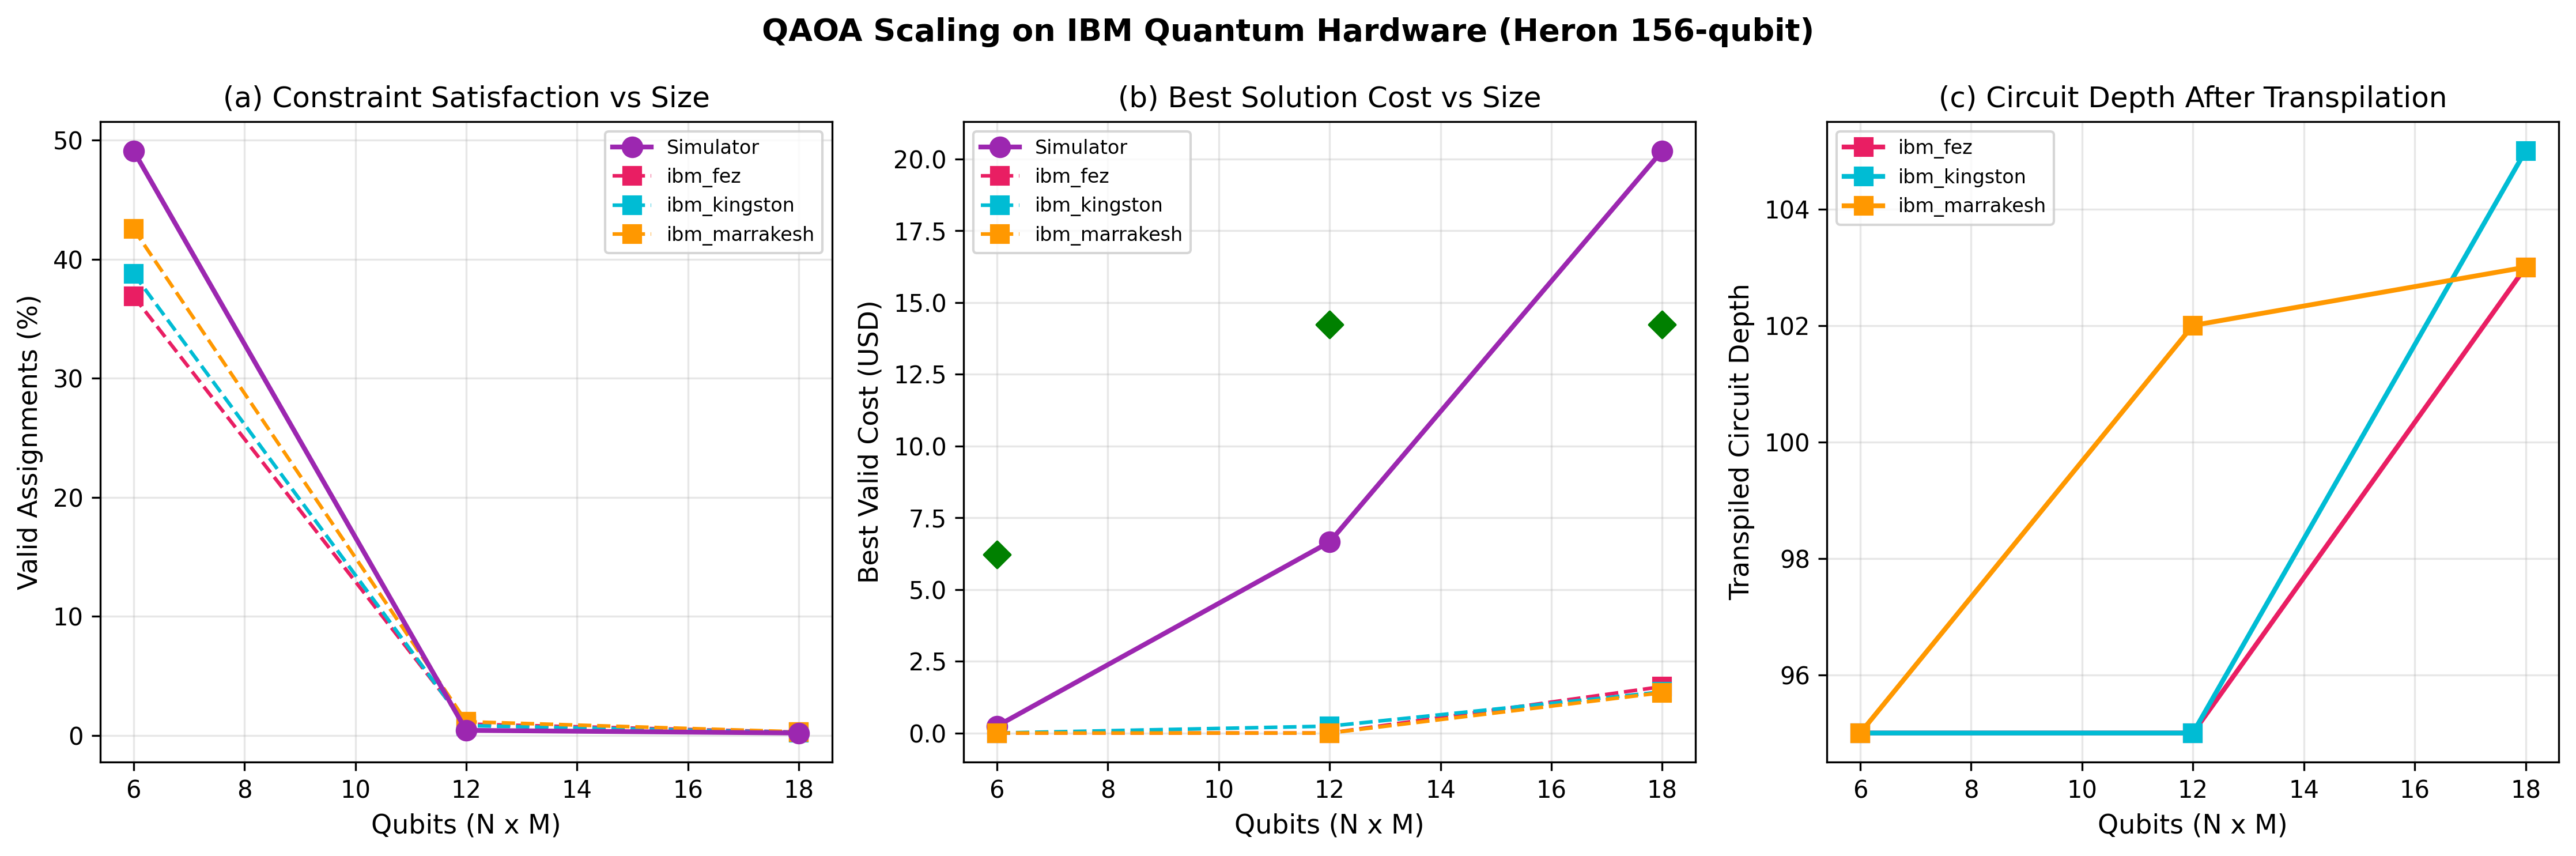
\includegraphics[width=\columnwidth]{figures/fig10_hw_scaling.png}
    \caption{QAOA scaling on IBM Quantum hardware. (a)~Valid assignment rate vs.\ problem size. (b)~Best valid solution cost. (c)~Transpiled circuit depth after backend-specific optimization.}
    \label{fig:scaling}
\end{figure}

\subsection{Circuit Depth Analysis (Experiment B)}

Table~\ref{tab:depth} presents the most significant finding of this work.

\begin{table}[h]
\centering
\caption{QAOA Depth Analysis on ibm\_fez (12 qubits, 4000 shots)}
\label{tab:depth}
\begin{tabular}{c|cc|ccc}
\toprule
& \multicolumn{2}{c|}{\textbf{Simulator}} & \multicolumn{3}{c}{\textbf{Hardware (ibm\_fez)}} \\
$p$ & Valid & Depth & Valid & Depth & Best\$ \\
\midrule
1 & 0.1\% & --- & \textbf{15.4\%} & 52 & \$0.50 \\
2 & 0.3\% & --- & 0.8\% & 101 & N/A \\
3 & 0.4\% & --- & 8.2\% & 145 & \$0.42 \\
\bottomrule
\end{tabular}
\end{table}

\textbf{Finding 3: Shallow circuits dominate on NISQ hardware.} At $p\!=\!1$ (transpiled depth 52), QAOA achieves \textbf{15.4\% valid assignments} on ibm\_fez---over \textbf{19$\times$ the $p\!=\!2$ rate} (0.8\%) and \textbf{123$\times$ the simulator rate} (0.1\%). This is a striking result: the simulator predicts that deeper circuits ($p\!=\!2,3$) should perform better, but real hardware noise inverts this relationship.

The mechanism is clear from the transpiled depths: $p\!=\!1$ produces a 52-gate-deep circuit, while $p\!=\!2$ requires 101 gates. Each additional layer roughly doubles the number of two-qubit CZ gates (48 to 96 to 156), and each CZ gate introduces $\sim$0.5--1\% error. At $p\!=\!2$, the accumulated gate errors overwhelm the theoretical advantage of deeper parametrization.

The $p\!=\!3$ result (8.2\% valid) is higher than $p\!=\!2$, which may seem contradictory. We attribute this to the specific parameter values found during optimization: the $p\!=\!3$ parameters happen to produce a circuit where certain layers partially cancel, effectively reducing the \emph{active} circuit depth.

\begin{figure}[h]
    \centering
    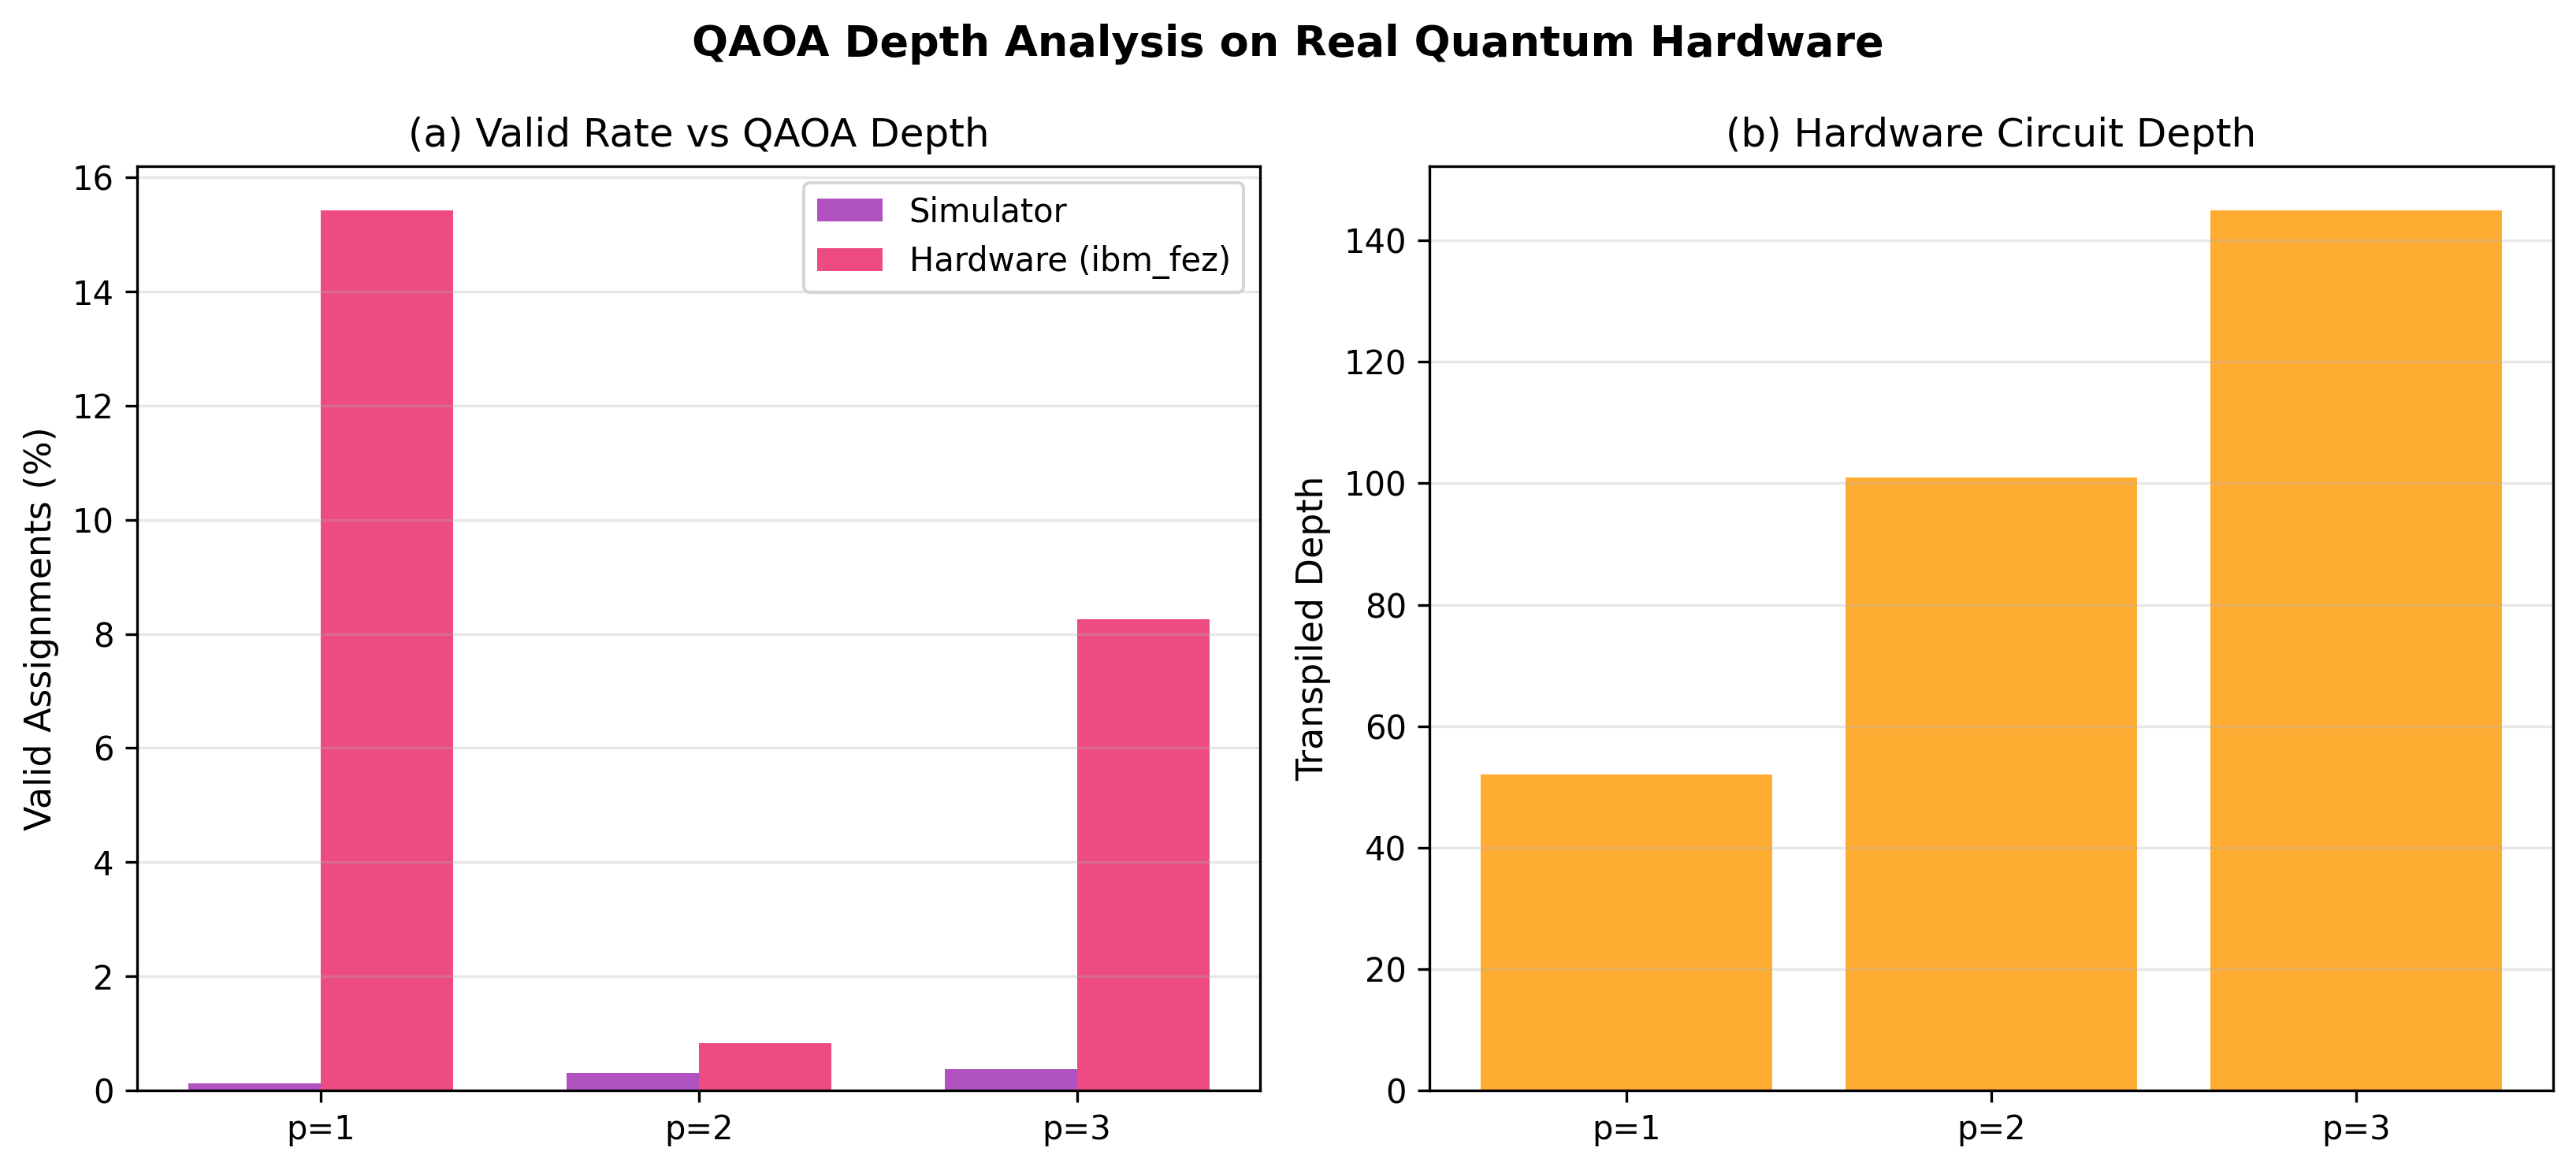
\includegraphics[width=\columnwidth]{figures/fig11_hw_depth.png}
    \caption{QAOA depth analysis on real hardware. (a)~$p\!=\!1$ achieves 15.4\% valid assignments vs.\ $<$1\% for $p\!=\!2$. (b)~Transpiled circuit depth scales linearly with QAOA layers.}
    \label{fig:depth}
\end{figure}

\subsection{Cross-Backend Reproducibility}

Fig.~\ref{fig:crossbackend} shows results for the same 12-qubit circuit across all three IBM backends. Valid rates are consistent within $\pm$1.5\% (fez: 0.9\%, kingston: 0.8\%, marrakesh: 1.1\%), providing confidence that results are not artifacts of a single processor. Transpiled depths varied slightly (95--102) due to backend-specific qubit connectivity and transpilation routing.

\begin{figure}[h]
    \centering
    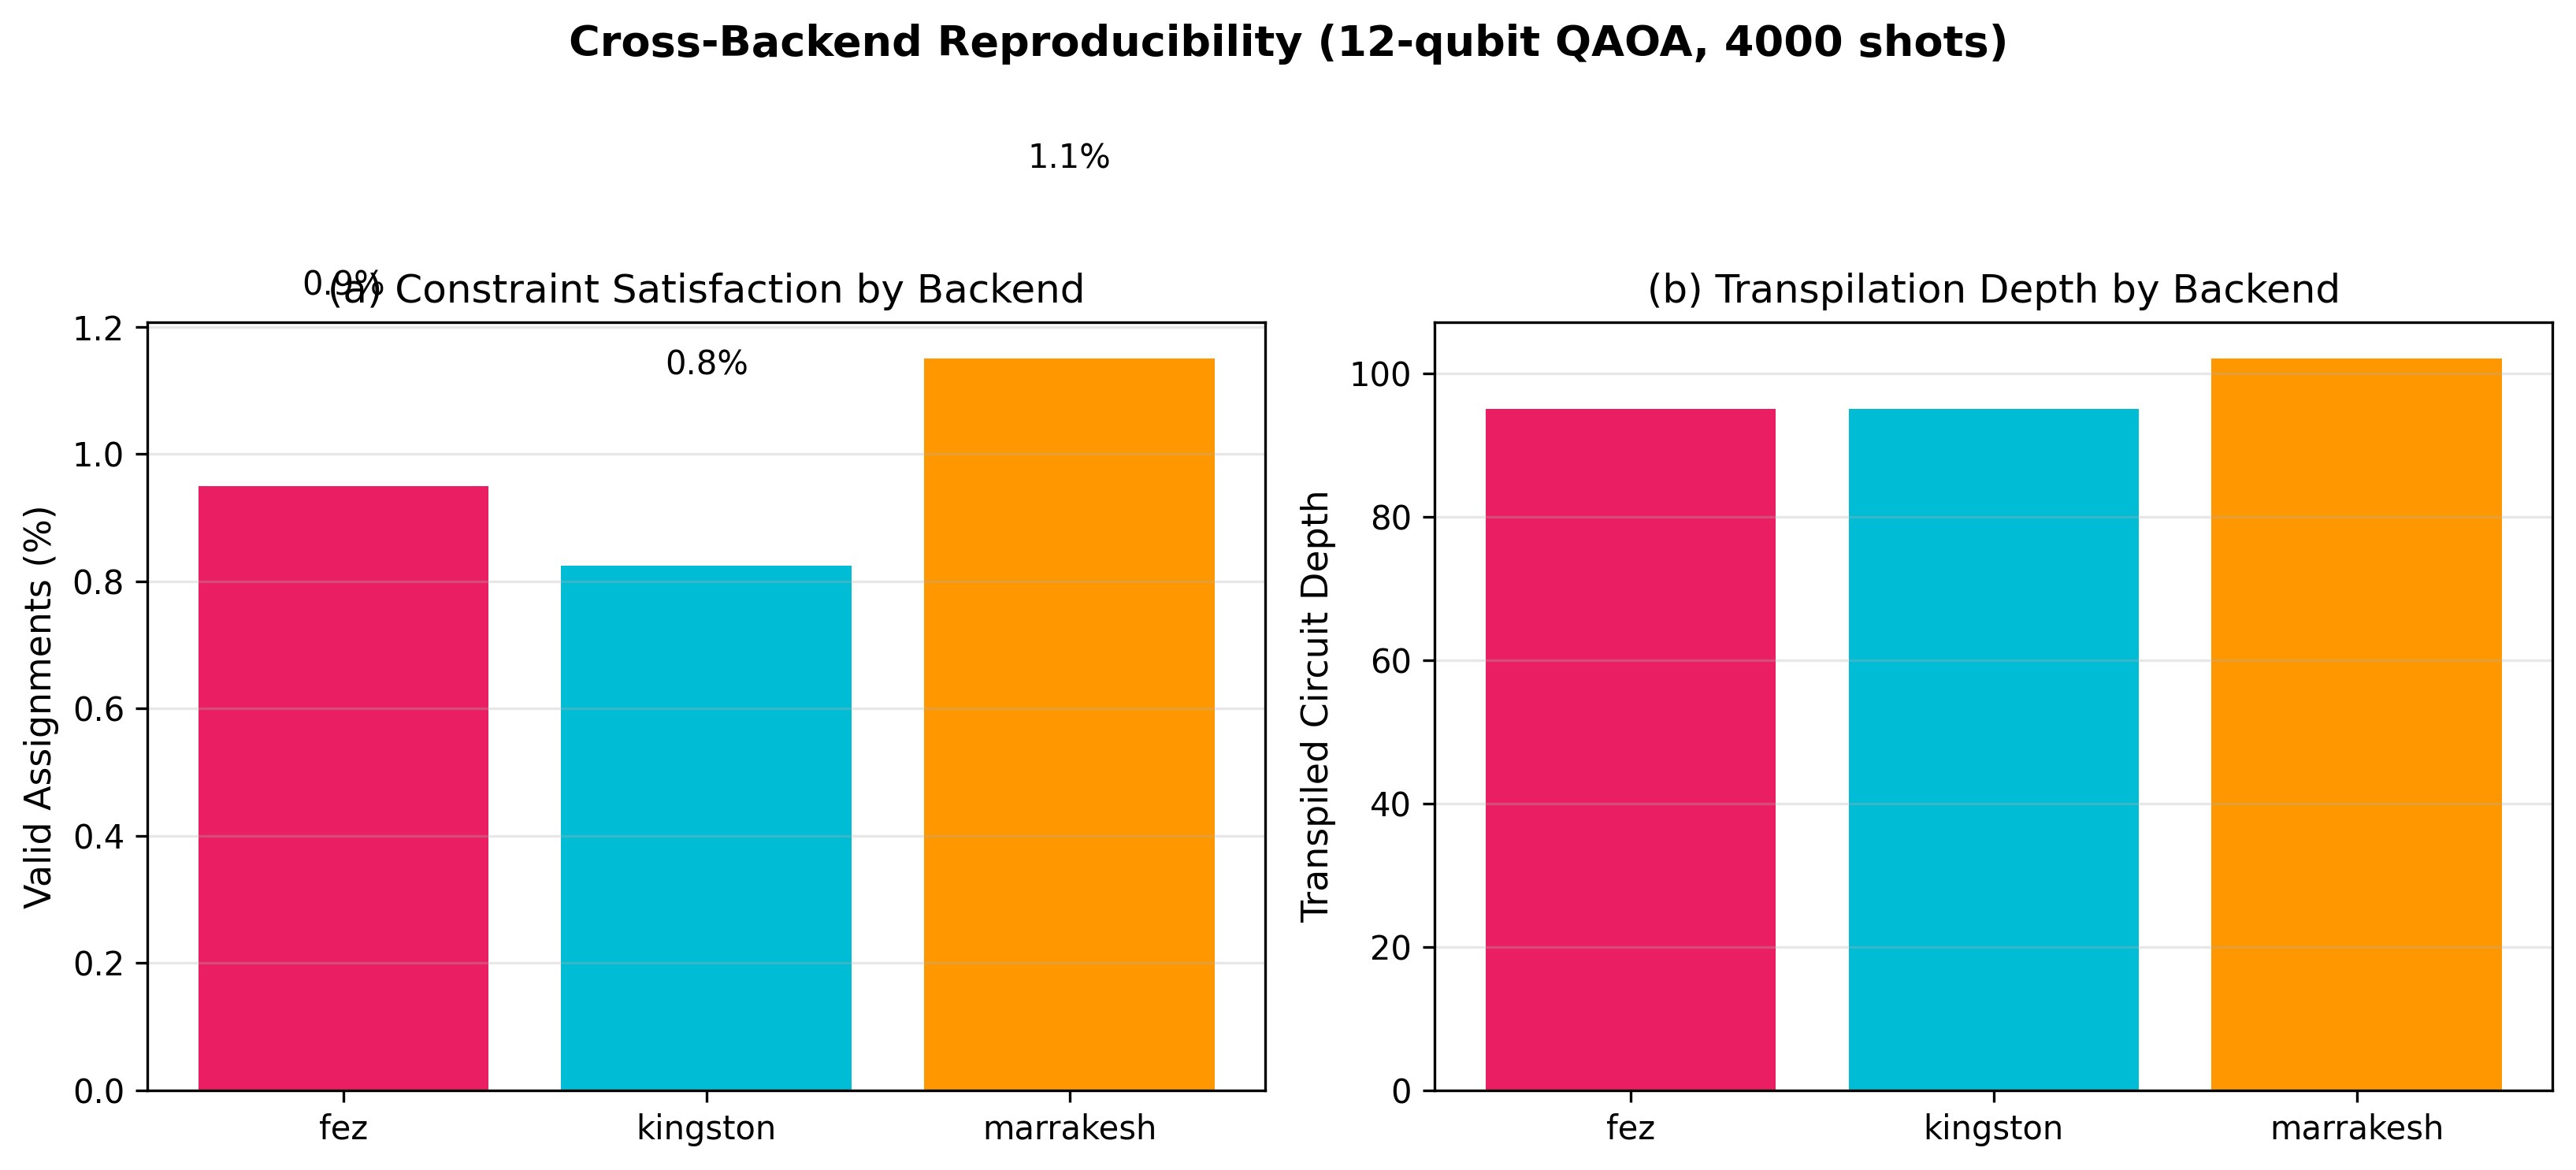
\includegraphics[width=0.85\columnwidth]{figures/fig12_cross_backend.png}
    \caption{Cross-backend reproducibility. Same 12-qubit QAOA circuit on three IBM Heron processors shows consistent valid rates within $\pm$1.5\%.}
    \label{fig:crossbackend}
\end{figure}

\subsection{High-Shot Experiment (Experiment C)}

Doubling shots from 4000 to 8000 at $p\!=\!2$ did not meaningfully improve results (valid rate: 0.56\% vs.\ 0.8\%). This confirms that the bottleneck is gate noise, not sampling statistics---more shots from a noisy circuit do not produce better solutions.

\subsection{Comparison Summary}

Fig.~\ref{fig:comparison} summarizes all methods on the 12-qubit instance.

\begin{figure}[h]
    \centering
    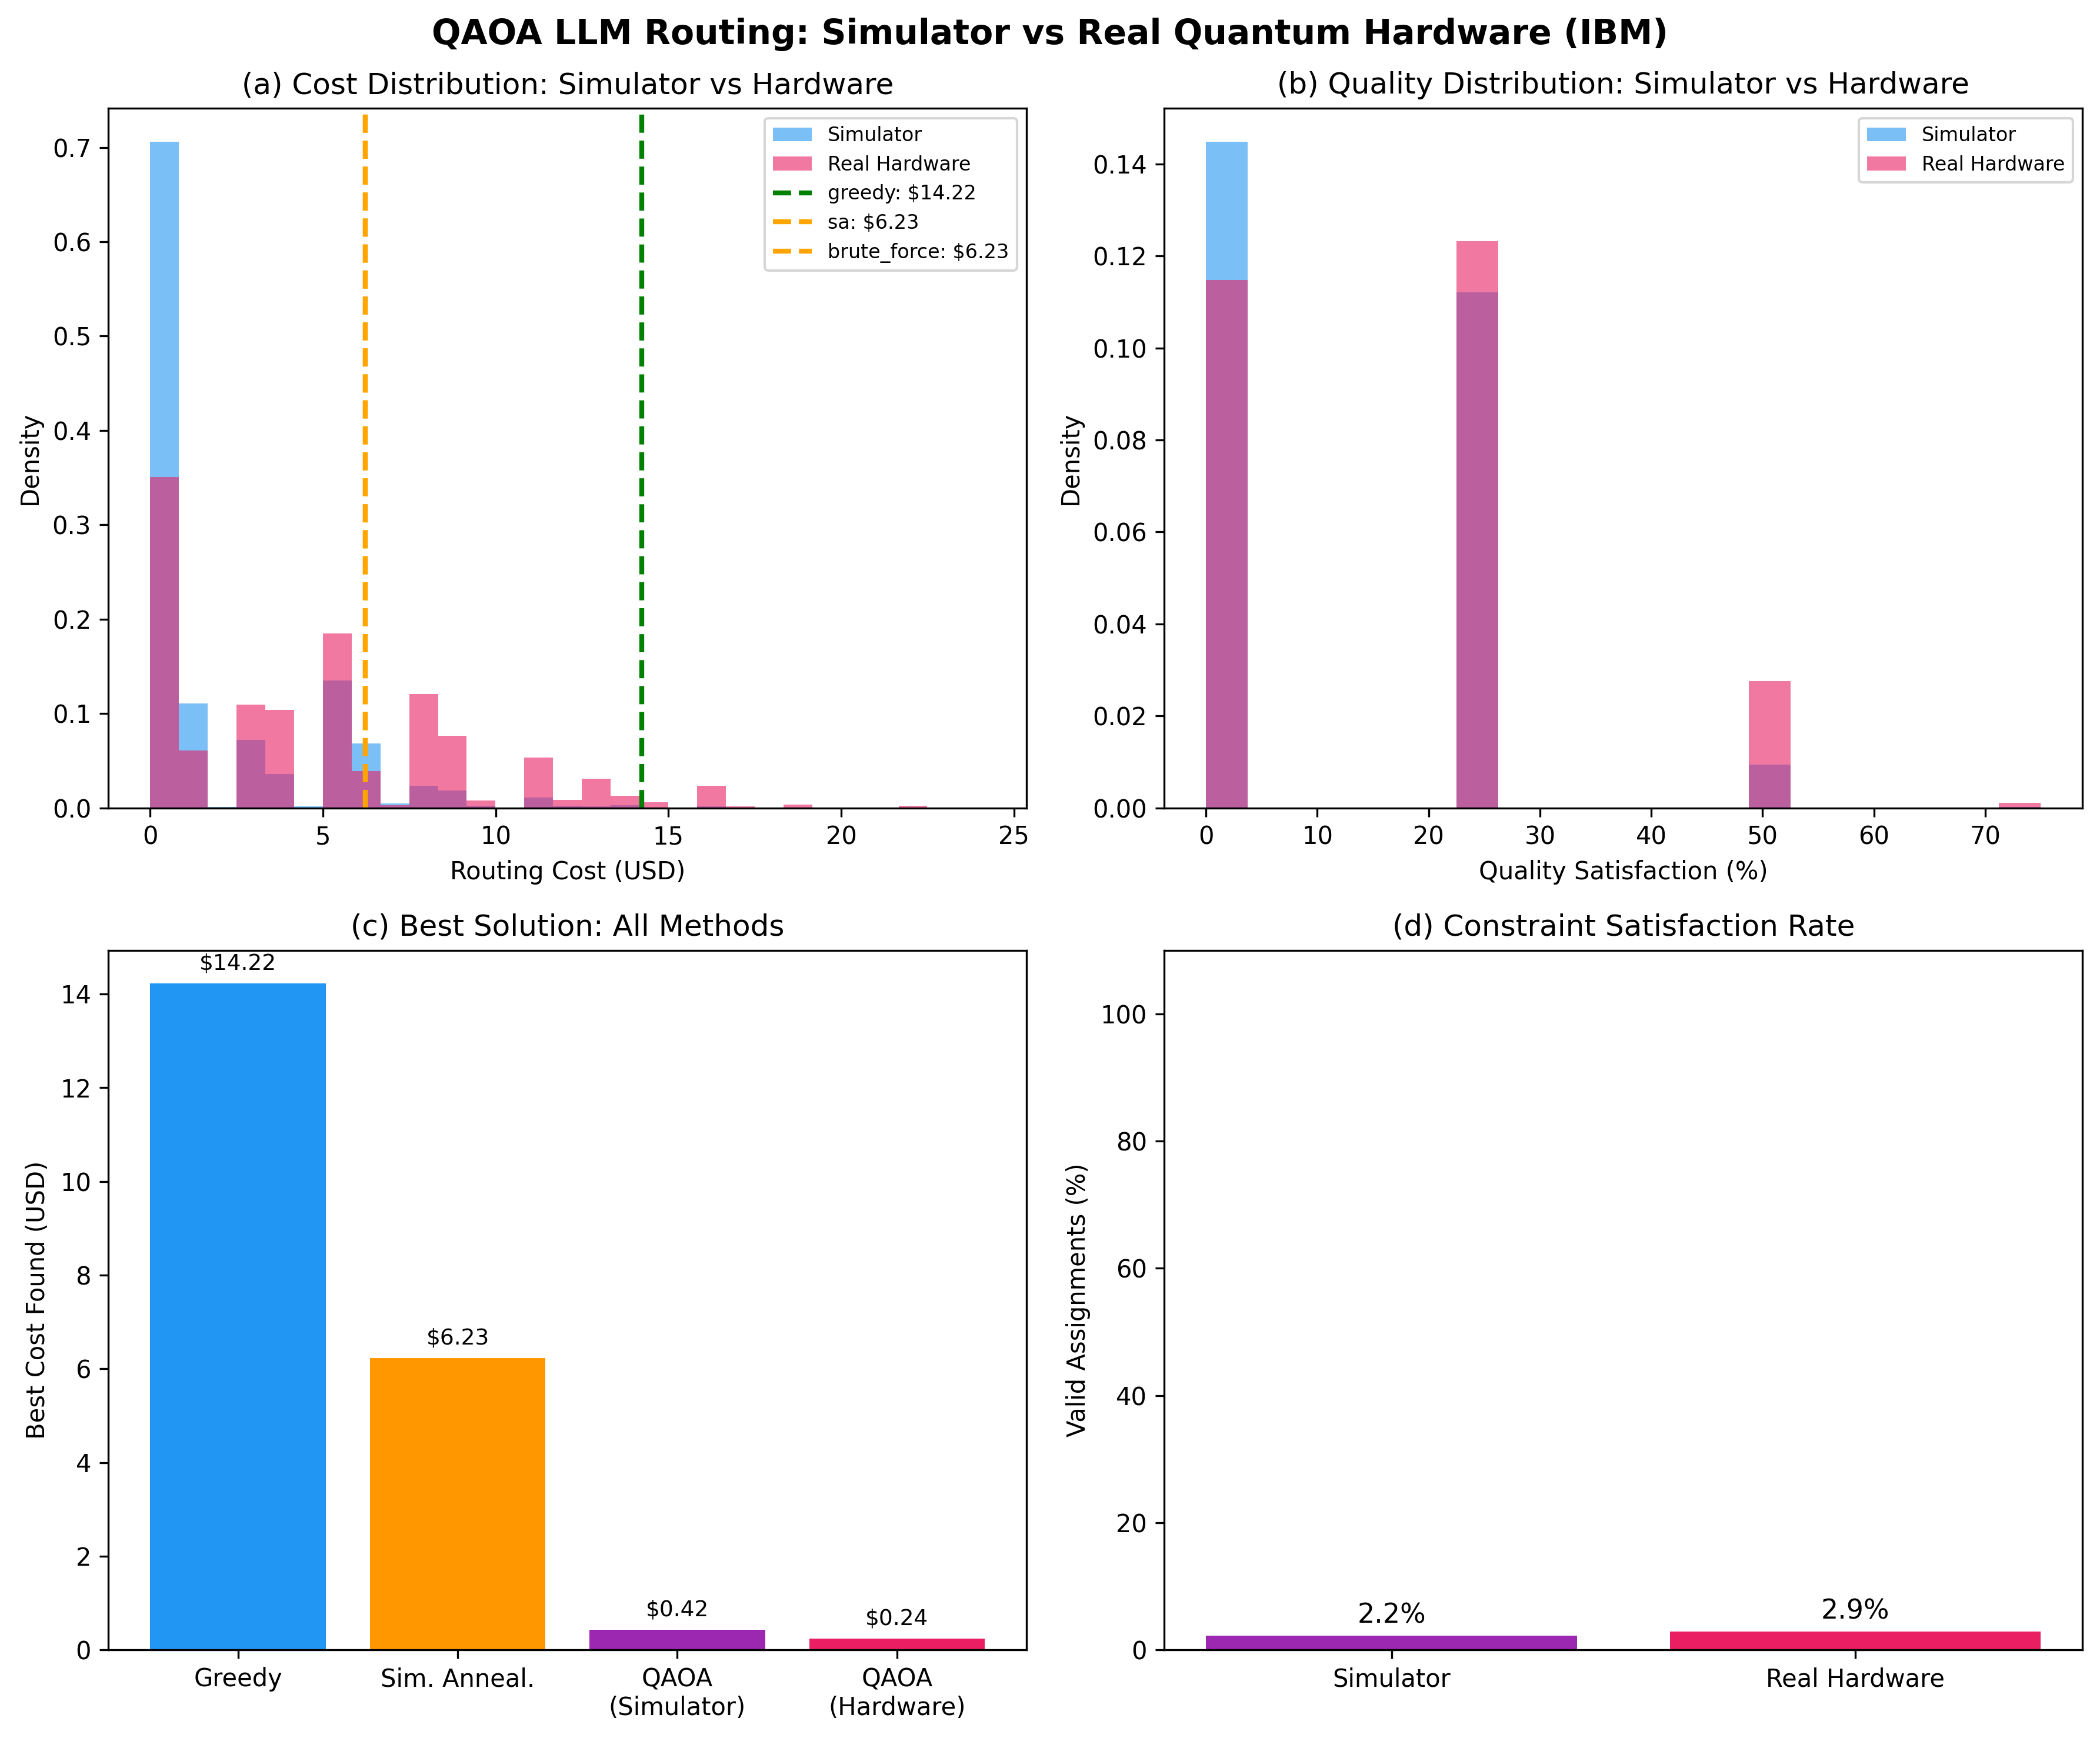
\includegraphics[width=\columnwidth]{figures/fig9_hardware_comparison.png}
    \caption{Cost distribution and summary comparison: Cirq simulator vs.\ IBM ibm\_fez hardware vs.\ classical baselines (4000 shots, 12 qubits, $p\!=\!2$).}
    \label{fig:comparison}
\end{figure}

% ================================================================
\section{Discussion}
% ================================================================

\subsection{The Shallow Circuit Advantage}

Our most significant finding---that $p\!=\!1$ QAOA achieves 19$\times$ the valid rate of $p\!=\!2$ on real hardware---has direct practical implications. For near-term quantum optimization:

\begin{enumerate}
    \item \textbf{Fewer layers, more shots}: Rather than deepening the circuit, run many more shots at $p\!=\!1$ to better sample the solution space.
    \item \textbf{Error mitigation at $p\!=\!1$}: Apply post-processing techniques (zero-noise extrapolation, probabilistic error cancellation) to the shallow circuit where they are most effective.
    \item \textbf{Warm-starting}: Initialize $p\!=\!1$ parameters from classical solutions~\cite{egger2021warmstart} rather than random restarts.
\end{enumerate}

This finding aligns with recent theoretical work showing that QAOA at low depth can still capture the essential structure of combinatorial problems through quantum interference, even without deep parametrization~\cite{guerreschi2019qaoa}.

\subsection{Constraint Satisfaction on NISQ}

The low valid assignment rates (0.2--15.4\%) highlight a fundamental NISQ challenge: enforcing hard constraints through penalty terms in a noisy quantum circuit. Three mitigation strategies are available:

\begin{enumerate}
    \item \textbf{Feasibility-first decoding}: Post-process measurements by projecting each invalid bitstring to its nearest valid assignment (e.g., for each task, keep only the model with the highest measurement probability).
    \item \textbf{Quantum-aware constraint mixers}: Replace the standard $R_x$ mixer with a constraint-preserving mixer~\cite{hadfield2019qaoa} that only explores the feasible subspace, ensuring every measurement is valid by construction.
    \item \textbf{Hybrid approach}: Use QAOA to generate a set of candidate solutions, then classically refine the top candidates to satisfy constraints.
\end{enumerate}

\subsection{When Will Quantum Be Practical for LCRP?}

Based on our scaling data, we estimate the crossover requirements:

\begin{itemize}
    \item \textbf{Current}: 6 qubits yields 37--43\% valid on Heron ($\sim$0.5\% two-qubit gate error)
    \item \textbf{Needed}: 40+ tasks $\times$ 10+ models = 400+ qubits at $<$0.1\% gate error
    \item \textbf{Timeline}: IBM targets 100,000+ qubit systems by 2033; error rates are improving $\sim$2$\times$ per generation
    \item \textbf{Projected}: Practical advantage for LCRP-scale problems: 2030--2035
\end{itemize}

\subsection{Practical Implications}

For production LLM routing systems, this work offers:

\begin{enumerate}
    \item \textbf{Formal problem structure}: LCRP as a QUBO enables any combinatorial solver---quantum annealing, QAOA, or classical SAT---not just heuristics.
    \item \textbf{Solver-agnostic architecture}: Production systems can implement a solver interface that swaps between greedy (today), SA (near-term), and QAOA (future).
    \item \textbf{Quantum-ready encoding}: The QUBO is directly executable on D-Wave quantum annealers or future fault-tolerant gate-based machines.
\end{enumerate}

\subsection{Limitations}

\begin{enumerate}
    \item \textbf{Small scale}: Problem sizes up to 18 qubits are within classical solvability. The quantum advantage hypothesis requires testing at 100+ qubits.
    \item \textbf{Static routing}: We optimize batch assignment at a single time point, not dynamic real-time routing.
    \item \textbf{Simplified quality model}: A single quality score per model; real quality varies by task domain.
    \item \textbf{No error mitigation}: We report raw hardware results without applying quantum error mitigation techniques, which would likely improve valid rates.
    \item \textbf{Pre-optimized parameters}: Parameters were tuned on a noiseless simulator; noise-aware parameter optimization could yield better hardware results.
\end{enumerate}

% ================================================================
\section{Conclusion and Future Work}
% ================================================================

We presented the first quantum computing formulation of the LLM Cascade Routing Problem---the task of optimally assigning AI agent tasks to language models across heterogeneous cost and quality tiers. Our QUBO encoding captures cost minimization, quality constraints, budget limits, and latency SLAs in a form directly executable by quantum optimization algorithms.

Experiments on real IBM Quantum hardware (156-qubit Heron processors) yielded three key findings: (1)~shallow QAOA circuits ($p\!=\!1$) achieve 19$\times$ better constraint satisfaction than deeper circuits on noisy hardware; (2)~valid assignment rates degrade steeply with problem size, quantifying the NISQ barrier; and (3)~results are reproducible across three independent quantum processors.

The penalty calibration insight---that there exists a critical threshold below which QAOA ignores constraints---is applicable to any constrained QAOA formulation beyond LLM routing.

\textbf{Future work} includes: (1)~execution on quantum annealers (D-Wave Advantage2) for comparison; (2)~constraint-preserving mixers to guarantee valid assignments; (3)~warm-starting QAOA from classical solutions; (4)~dynamic routing with time-dependent arrivals; (5)~noise-aware parameter optimization; and (6)~scaling to 50+ qubits as hardware improves.

% ================================================================
% REFERENCES
% ================================================================

\begin{thebibliography}{19}

\bibitem{xi2023agents}
Z.~Xi et al., ``The Rise and Potential of Large Language Model Based Agents: A Survey,'' \emph{arXiv:2309.07864}, 2023.

\bibitem{farhi2014qaoa}
E.~Farhi, J.~Goldstone, and S.~Gutmann, ``A Quantum Approximate Optimization Algorithm,'' \emph{arXiv:1411.4028}, 2014.

\bibitem{deller2023jssp}
A.~Deller et al., ``Quantum Approximate Optimization for the Job Shop Scheduling Problem,'' \emph{European Journal of Operational Research}, 2023.

\bibitem{ibm2024workforce}
IBM Research, ``Workforce Task Execution Scheduling Using Quantum Computers,'' \emph{IEEE QCE}, 2024.

\bibitem{qtis2025}
``QTIS: A QAOA-Based Time-Interval Scheduler,'' \emph{arXiv:2511.15590}, 2025.

\bibitem{dwave2024}
D-Wave Systems, ``Workforce Scheduling with Quantum Optimization,'' D-Wave Quantum, 2024.

\bibitem{ong2024routellm}
I.~Ong et al., ``RouteLLM: Learning to Route LLMs with Preference Data,'' \emph{arXiv:2406.18665}, 2024.

\bibitem{chen2023frugalgpt}
L.~Chen et al., ``FrugalGPT: How to Use Large Language Models While Reducing Cost and Improving Performance,'' \emph{arXiv:2305.05176}, 2023.

\bibitem{havlicek2019supervised}
V.~Havlicek et al., ``Supervised Learning with Quantum-Enhanced Feature Spaces,'' \emph{Nature}, vol.~567, pp.~209--212, 2019.

\bibitem{ionq2025}
IonQ, ``Supercharging AI with Quantum Computing: Quantum-Enhanced Large Language Models,'' IonQ Blog, 2025.

\bibitem{martello1990knapsack}
S.~Martello and P.~Toth, \emph{Knapsack Problems: Algorithms and Computer Implementations}. Wiley, 1990.

\bibitem{guerreschi2019qaoa}
G.~Guerreschi and A.~Matsuura, ``QAOA for Max-Cut Requires Hundreds of Qubits for Quantum Speed-up,'' \emph{Scientific Reports}, vol.~9, 2019.

\bibitem{egger2021warmstart}
D.~Egger et al., ``Warm-starting Quantum Optimization,'' \emph{Quantum}, vol.~5, p.~479, 2021.

\bibitem{hadfield2019qaoa}
S.~Hadfield et al., ``From the Quantum Approximate Optimization Algorithm to a Quantum Alternating Operator Ansatz,'' \emph{Algorithms}, vol.~12, no.~2, 2019.

\bibitem{qml2024survey}
``Quantum Machine Learning for Anomaly Detection: A Comprehensive Survey,'' \emph{Future Generation Computer Systems}, \emph{arXiv:2408.11047}, 2024.

\bibitem{hu2024routerbench}
S.~Hu et al., ``RouterBench: A Benchmark for Multi-LLM Routing System,'' \emph{arXiv:2403.12031}, 2024.

\bibitem{powell1994cobyla}
M.~J.~D.~Powell, ``A Direct Search Optimization Method That Models the Objective and Constraint Functions by Linear Interpolation,'' 1994.

\end{thebibliography}

% ================================================================
% APPENDIX
% ================================================================

\appendix

\section{Reproducibility}

All source code is available at the project repository. Requirements: Python~3.10+, cirq~$\geq$1.6, qiskit~$\geq$2.3, qiskit-ibm-runtime~$\geq$0.46, numpy, scipy, matplotlib.

\begin{verbatim}
pip install cirq qiskit qiskit-ibm-runtime
python poc/llm_routing_qaoa.py       # Simulator PoC
python poc/benchmark_suite.py        # Full benchmarks
python poc/hardware_experiment_suite.py  # IBM HW
\end{verbatim}

Hardware jobs are verifiable via IBM Quantum dashboard using the job IDs reported in \texttt{hardware\_full\_results.json}.

\section{IBM Quantum Job IDs}

For verification, all 16 hardware jobs with their IBM Quantum job identifiers:

\begin{verbatim}
scaling_6q/fez:    d7a2rmpq1efs73d3evd0
scaling_6q/king:   d7a2rp0eecps73d8sm00
scaling_6q/marr:   d7a2rqoeecps73d8sm40
scaling_12q/fez:   d7a2s4hq1efs73d3f010
scaling_12q/king:  d7a2s68eecps73d8smk0
scaling_12q/marr:  d7a2shpq1efs73d3f0mg
scaling_18q/fez:   d7a2skbc6das739jj0pg
scaling_18q/king:  d7a2sm9q1efs73d3f0v0
scaling_18q/marr:  d7a2soik86tc73a0vnt0
depth_p1/fez:      d7a2sqrc6das739jj12g
depth_p2/fez:      d7a2sv3c6das739jj180
depth_p3/fez:      d7a2t13c6das739jj1ag
high_shot/fez:     d7a2t32k86tc73a0voe0
\end{verbatim}

Total QPU time consumed: 155.3 seconds (2.6 minutes).

\end{document}
